\section{Estructuras de contención} % (fold)
\label{sec:estructuras_de_contención}

\subsection{Muros de gravedad} % (fold)
\label{sub:muros_de_gravedad}

\begin{mydef}[Regla del núcleo central]
	Corresponde a la condición de no existencia de tracciones (suponiendo una distribución lineal). No es restristictiva se puede prescindir de ella en casos de terrenos duros (arcillas duras, rocas…). Ocurre si el punto de aplicación de la resultante respecto la base es :
	\[
		e> \frac{B}{6}
	\]
\end{mydef}


\subsection{Pantallas} % (fold)
\label{sub:pantallas}

\begin{mybox}{Pantallas}
	Son estructuras esbeltas, construidas con material que resiste a la tracción (acero, hormigón armado)
	\tcbsubtitle{\emph{Tablestacas}}

	\begin{minipage}[t]{0.5\textwidth}
	Ventajas:
	\begin{enumerate}
		\item Flexibles
		\item Estancas
		\item Reutilización fácil
	\end{enumerate}
	\end{minipage}%
	\begin{minipage}[t]{0.5\textwidth}
	Inconvenientes:
		\begin{itemize}
			\item Limitación de longitud
			\item Corrosión
			\item Difíciles de soldar
			\item No se pueden instalar en cualquier terreno
		\end{itemize}
	\end{minipage}

	\tcbsubtitle{\emph{Hormigonadas ``in-situ''}}
	Problemas comunes:
	\begin{itemize}
		\item Fallos de hormigonado (mala colocación)
		\item Fallos de inyección (falta adherencia)
		\item Mala calidad de los materiales
	\end{itemize}

	\tcbsubtitle{\emph{Otros tipos de pantallas}}
	\begin{itemize}
		\item Pilotes
		\item Micro-pilotes
		\item Damas
		\item Entibaciones
	\end{itemize}

	\tcbsubtitle{\emph{Posibles modos de fallo}}

	\tcbsubtitle{\emph{Estado tensional en voladizo}}

	\begin{minipage}[t]{0.5\textwidth}
	\begin{figure}[H]
		\centering
		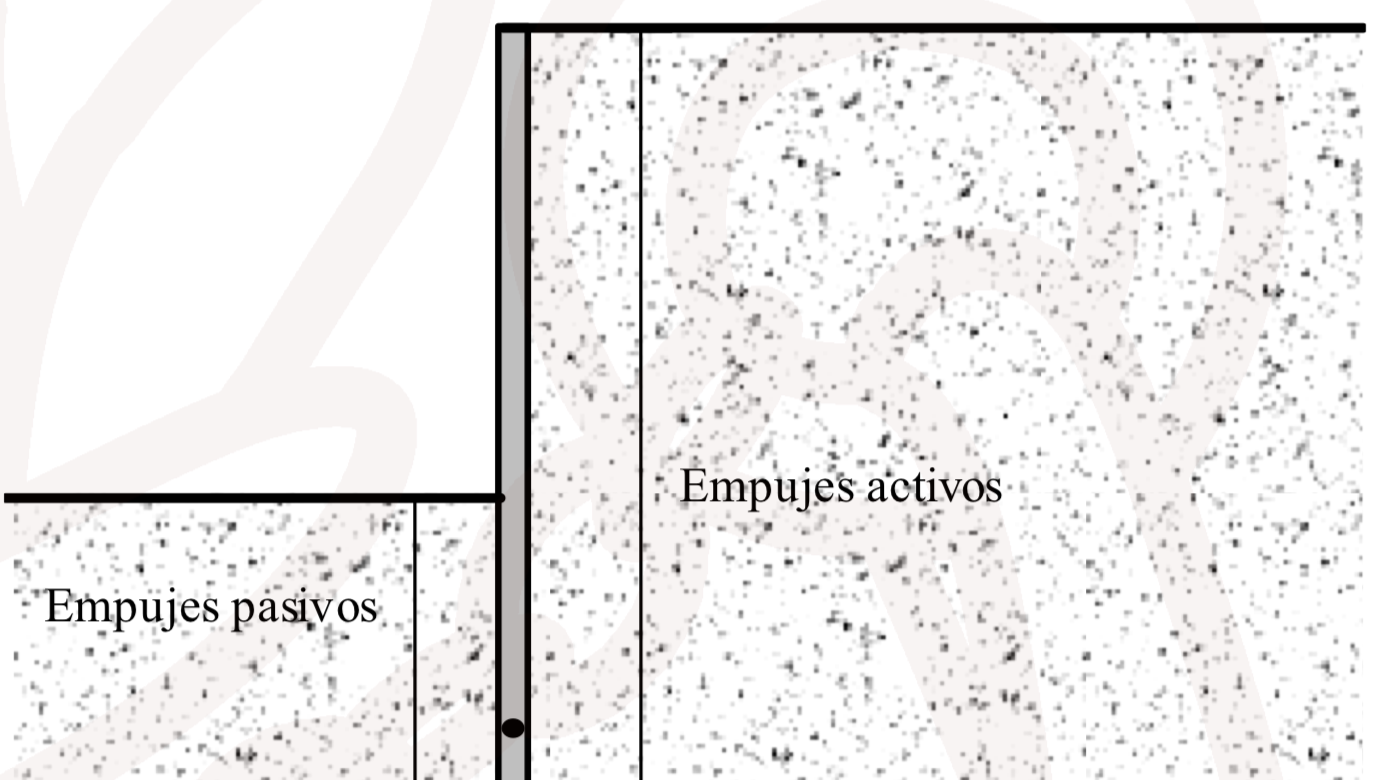
\includegraphics[width=0.95\textwidth]{img/confi1}
		\caption{Estado tensional 1 (translación)}
		\label{fig:confi1}
	\end{figure}
	\end{minipage}%
	\begin{minipage}[t]{0.5\textwidth}
	\begin{figure}[H]
		\centering
		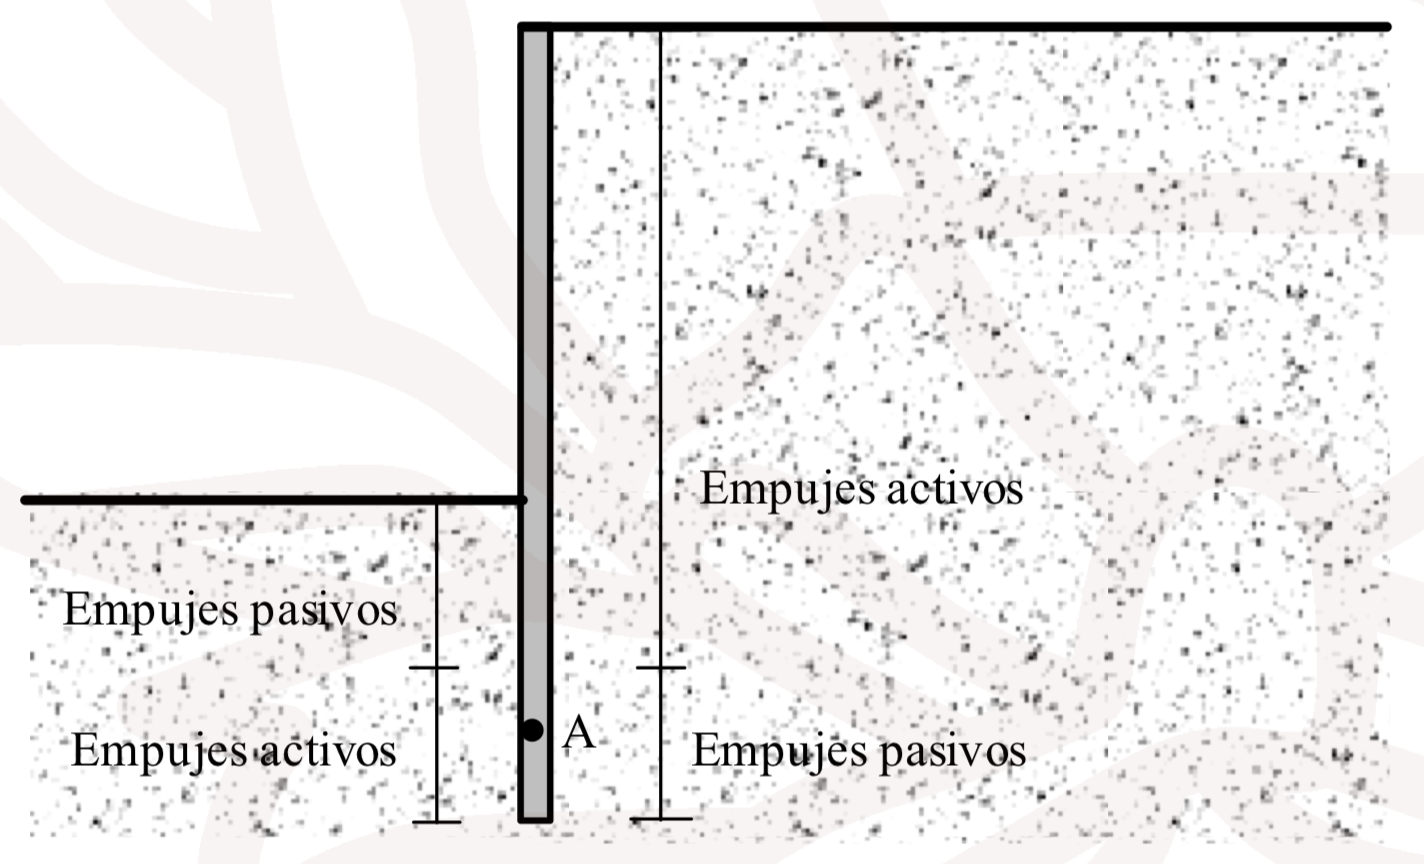
\includegraphics[width=0.95\textwidth]{img/confi2}
		\caption{Estado tensional 2 (rotación)}
		\label{fig:confi2}
	\end{figure}
	\end{minipage}

	\tcbsubtitle{\emph{Métodos de análisis}}

	\paragraph{En voladizo} % (fold)
	\label{par:en_voladizo}

	Sólo podemos analizar el caso de la Figure~\ref{fig:confi2} ya que la Figure~\ref{fig:confi1} no es estable.
	
	\begin{figure}[H]
		\centering
		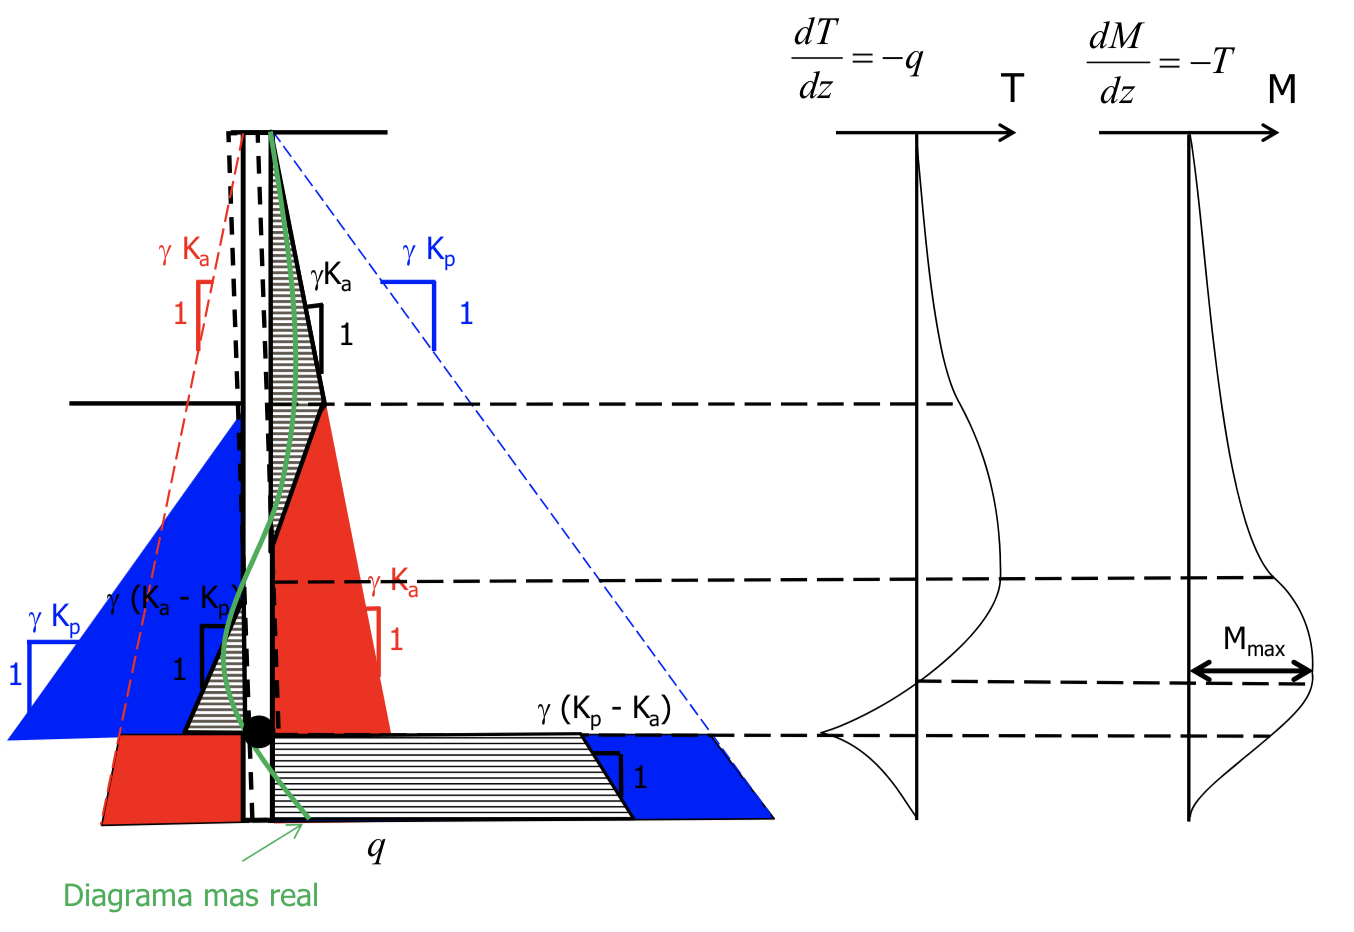
\includegraphics[width=0.95\textwidth]{img/voladizo}
		\caption{Análisis voladizo}
		\label{fig:voladizo}
	\end{figure}
	% paragraph en_voladizo (end)

	\paragraph{Soporte libre} % (fold)
	\label{par:soporte_libre}
	El estado tensional es cómo Figure~\ref{fig:confi1}. Este método considera que la profundidad del empotramiento es pequeña o que la rigidez de la pantalla es grande. Se asume que la pantalla se desplaza de una manera rígida bajo el efecto de la \emph{presión activa} de tierras y moviliza la presión pasiva a lo largo de su parte empotrada. Se considera que no hay reacción en la base. Es un sistema isostático no necesitamos hipótesis adicionales.
	\begin{figure}[H]
		\centering
		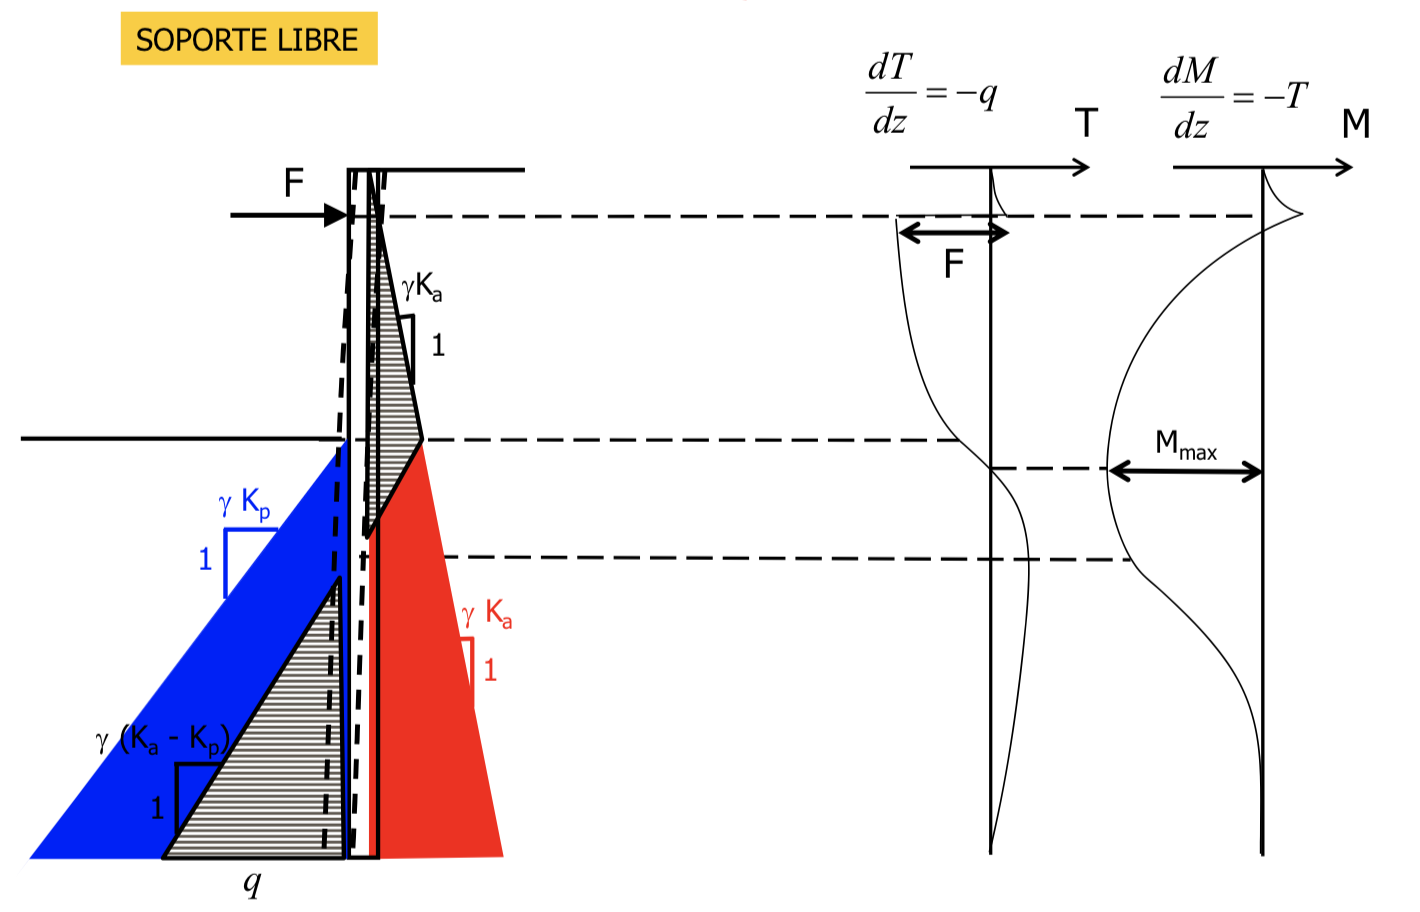
\includegraphics[width=0.95\textwidth]{img/soporte_libre}
		\caption{Análisis soporte libre}
		\label{fig:soporte_libre}
	\end{figure}
	% paragraph soporte_libre (end)

	\paragraph{Soporte fijo} % (fold)
	\label{par:soporte_fijo}
	El estado tensional es cómo la Figure~\ref{fig:confi2}. Este método considera que la rigidez es pequeña o la profundidad del empotramiento grande. Se considera que la base está empotrada. Este sistema es hiperestático, así pues es necesario realizar la hipótesis siguiente para resolverlo.
	\[
		x | \ q=0 \Leftrightarrow T(x) = T_{max} := M(x)=0
	\]
	\begin{figure}[H]
		\centering
		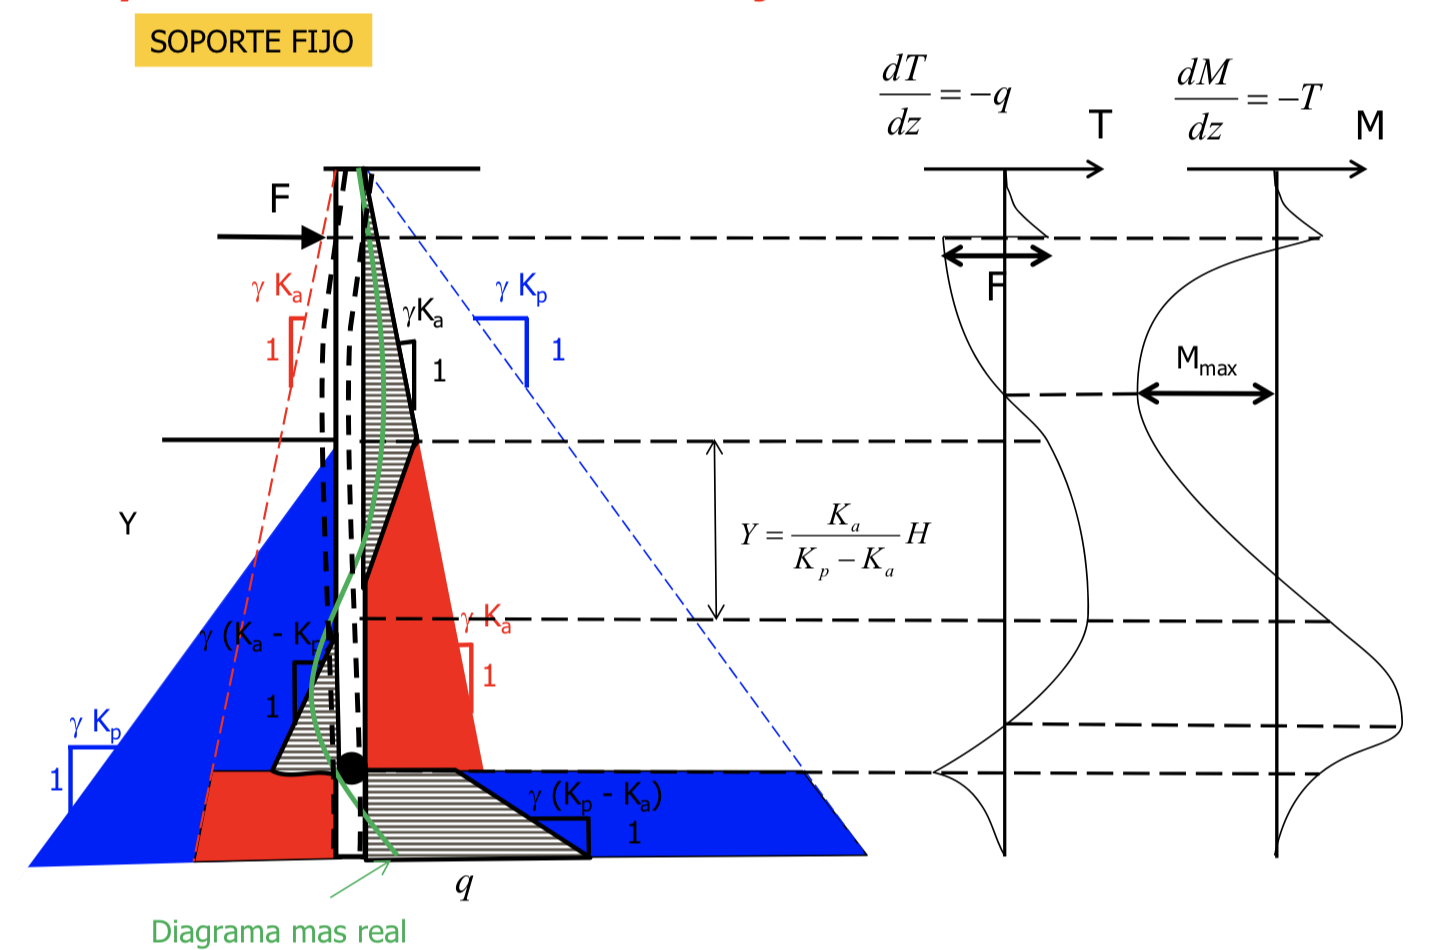
\includegraphics[width=0.95\textwidth]{img/soporte_fijo}
		\caption{Análisis soporte fijo}
		\label{fig:soporte_fijo}
	\end{figure}
	% paragraph soporte_fijo (end)
\end{mybox}

\begin{mybox}{Tierra reforzada}
	No requieren cimentación, tienen un buen comportamiento en suelos de mala calidad y permiten alturas importantes ($h>20m$)
	\begin{minipage}[t]{0.5\textwidth}
	Ventajas:
	\begin{enumerate}
		\item Estructura flexible (se adapta a asientos importantes en cimentación)
		\item Ejecución rápida con material ligero
		\item Coste competitivo
		\item Se pueden alcanzar alturas importantes
	\end{enumerate}
	\end{minipage}%
	\begin{minipage}[t]{0.5\textwidth}
	Inconvenientes:
		\begin{itemize}
			\item Relleno debe ser de calidad
			\item Problemas de durabilidad (corrosión de armaduras)
		\end{itemize}
	\end{minipage}
	\tcbsubtitle{\emph{Posibles modos de fallo}}

	\begin{enumerate}
		\item Por rotura a tracción de la armadura
		\item Por falta de adherencia armadura-relleno en la zona resistente
	\end{enumerate}

	\tcbsubtitle{\emph{Condiciones de estabilidad}}
	\begin{enumerate}
		\item Rotura a tracción:
		\[
			T_M \leq \frac{1}{F_1}\sigma_r b e
		\]
		\item Adherencia:
		\[
			T_M^{*}\leq \frac{1}{F_2}\int_0^{2a}\mu^* \sigma_v(x)2bdx
		\]

	\end{enumerate}
	Cálculo de la tracción máxima:
	\[
		T_M = \frac{1}{n}\sigma_h \Delta H
	\]
\end{mybox}

% subsection pantallas (end)
% subsection muros_de_gravedad (end)
% section estructuras_de_contención (end)